\documentclass[12pt,a4paper,oneside]{book}
\usepackage[utf8]{inputenc}
\usepackage[ngerman]{babel}
\usepackage[T1]{fontenc}
\usepackage[nohyperlinks, printonlyused]{acronym}

% Hauptdatei des Projektes. Von hier aus werden die anderen Seiten eingebunden
\usepackage{amsmath}
\usepackage{amsfonts}
\usepackage{amssymb}
\usepackage{xspace}
\usepackage[normalem]{ulem}
\usepackage{graphicx}
\usepackage{color, colortbl}
\usepackage[table]{xcolor}
\usepackage{nicefrac}
\usepackage{float}


%https://tex.stackexchange.com/questions/97474/how-to-add-lstlistoflistings-to-the-table-of-contents
\usepackage[nottoc]{tocbibind}

%%%%%%%%%%%%%%%%%%%%%%%%%%%%%%%%%%%%%%%%%%%%%%%%%%%%%%%%%%%%%%%%%%%%%%%%%%%%%%%%%%%%%%%%%%
% In diesem Abschnitt gibst du deine persönlichen Daten sowie den Kontext deiner Arbeit an
% das \xspace am Ende der Einträge muss vorhanden bleiben. Es regelt das Whitespace-
% handling
%%%%%%%%%%%%%%%%%%%%%%%%%%%%%%%%%%%%%%%%%%%%%%%%%%%%%%%%%%%%%%%%%%%%%%%%%%%%%%%%%%%%%%%%%%
% persönliche Daten
%\newcommand{\vorname}{Markus\xspace}
%\newcommand{\nachname}{Schäfer\xspace}
%\newcommand{\emailadresse}{markus.schaefer@et.hs-fulda.de\xspace}
%\newcommand{\matrikelnummer}{945228\xspace}


% Arbeitsspezifische Daten
\newcommand{\titel}{mail@kitanet\xspace}
\newcommand{\untertitel}{Implementierung eines internen E-Mail-Dienstes als Funktionserweiterung eines sozialen Netzwerkes\xspace}
\newcommand{\modulname}{Bachelor-Thesis\xspace}
\newcommand{\pruefer}{Prof. Dr. Uwe Werner\xspace}
\newcommand{\zweitpruefer}{Dipl. Ing. Rouven Braden\xspace}
\newcommand{\semester}{WiSe 2021\xspace}
\newcommand{\ortderarbeit}{Ockenheim\xspace}
%%%%%%%%%%%%%%%%%%%%%%%%%%%%%%%%%%%%%%%%%%%%%%%%%%%%%%%%%%%%%%%%%%%%%%%%%%%%%%%%%%%%%%%%%%

%Um einzelne Seite im Querformat zu verwenden
\usepackage{pdflscape}

% Damit Tabellen über die ganze Seitenbreite gehen
% https://texwelt.de/wissen/fragen/446/wie-bekomme-ich-eine-tabelle-in-textbreite
\usepackage{booktabs}
\usepackage{tabularx}
% Abstand zwischen Tabelle und Überschrift
% http://www.chemieonline.de/forum/showthread.php?t=101576
%\setlength{\belowcaptionskip}{0.3em}
\usepackage[center]{caption}
\newcommand*{\thead}[1]{\multicolumn{1}{c}{\bfseries #1}}
       
\usepackage{tikz}
\usepackage{pgfplots, pgfplotstable}

%Hurenkinder uns Schusterjungen
\clubpenalty10000
\widowpenalty10000
\displaywidowpenalty=10000

\usepackage{hyperxmp} % XMP-Daten fuer die PDF-Datei
%Gimmmick: Linked Kapitel und Inhaltsverzeichnis, sowie Referenzen
\usepackage[pdftex, pdfa]{hyperref}
\hypersetup{
    colorlinks,
    citecolor=black,
    filecolor=black,
    linkcolor=black,
    urlcolor=black,    
    pdftitle = {\titel},
    %pdfauthor = {\vorname \nachname},
    pdfsubject = {\untertitel},
    pdfkeywords = {\titel \untertitel},
    pdflang = de,
    %bookmarks = true,
    pdfdisplaydoctitle = true,
    colorlinks = true,
    plainpages = false,
    %allcolors = black,
    hypertexnames = false,
    %pdfpagelabels = true,
    %hyperindex = true,
    unicode = true,
   % pdfcaptionwriter = {\textsl{\vorname \nachname}},
   % pdfcontactaddress = {In den Weider 4},
   % pdfcontactcity = {Ockenheim},
   % pdfcontactpostcode = {55437},
    pdfcontactcountry = {Deutschland},
   % pdfcontactregion = {RLP},
   % pdfcontactemail = {\emailadresse},
   % pdfcontactphone = {0176/20479746},
    pdfcontacturl = {http://www.hs-fulda.de},
    pdfmetalang = {de},
}

\usepackage{prettyref}
\usepackage{titleref}

%Schriftart

%\renewcommand*\rmdefault{cmdh}
%\usepackage{lmodern}
%\usepackage{mathptmx}
%\usepackage[scaled=.90]{helvet}
%\usepackage{courier}
%\usepackage{bera}
%\usepackage{boisik}

%Inhaltsverzeichnis
\usepackage[tocgraduated]{tocstyle}
\usetocstyle{allwithdot}
\setcounter{tocdepth}{3}

% Formatierungshilfen: http://wwws.htwk-leipzig.de/~myagovki/latex/formatierungshilfen/

\usepackage[ddmmyyyy]{datetime}
\renewcommand{\dateseparator}{.}


% Für Kopf und Fußzeile: https://esc-now.de/_/latex-individuelle-kopf--und-fusszeilen/?lang=en
\usepackage[
  headsepline, plainheadsepline,
  footsepline, plainfootsepline
]{scrlayer-scrpage}
\pagestyle{scrheadings}
\clearscrheadfoot

    
\ihead*{
   \itshape \leftmark
}
%\ohead*{\vorname \nachname}
\ifoot*{\today}
\ofoot*{\pagemark}





% anderthalbfacher Zeilenabstand
\usepackage[onehalfspacing]{setspace}

%Geometry der Seite festlegen
\usepackage{geometry}
\geometry{
  left=2.5cm,
  right=2.5cm,
  top=2.5cm,
  bottom=2.5cm,
  headheight=33pt
}

%Für Gestaltung des Layouts
\usepackage{blindtext}

%Bilbliothek und Literatur einbinden
\usepackage[style=authoryear-ibid,natbib=true,bibencoding=utf8,backend=biber,sorting=nty]{biblatex}
\usepackage[babel,german=guillemets]{csquotes}
\defbibheading{head}{{\chapter*{Literaturverzeichnis}\addcontentsline{toc}{chapter}{Literaturverzeichnis}}}
\addbibresource{bib/literatur.bib}

%https://texwelt.de/fragen/19153/pdf-dateien-in-anhang-einbinden-aber-formatierung-des-vorhergehenden-dokuments-ubernehmen
\usepackage{pdfpages}

\newcommand{\zb}{z.\,B.\xspace}
\newcommand{\ua}{u.\,a.\xspace}
\newcommand{\oge}{o.\,g.\xspace}
\newcommand{\dah}{d.\,h.\xspace}
\newcommand{\bzw}{bzw.\xspace}
\newcommand{\bzgl}{bzgl.\xspace}
\newcommand{\ggf}{ggf.\xspace}
\newcommand{\bspw}{beispielsweise\xspace}

%https://stackoverflow.com/questions/3175105/writing-code-in-latex-document
\newcommand{\code}[1]{\texttt{#1}}

%https://tex.stackexchange.com/questions/115467/listings-highlight-java-annotations
\usepackage{listings}
\usepackage{inconsolata}

\usepackage{color}

\definecolor{pblue}{rgb}{0.13,0.13,1}
\definecolor{pgreen}{rgb}{0,0.5,0}
\definecolor{pgrey}{rgb}{0.46,0.45,0.48}
\definecolor{mauve}{rgb}{0.58,0,0.82}

\usepackage{listings}

\lstset{
  frame=t,
  language=bash,
  aboveskip=1mm,
  belowskip=1mm,
  columns=flexible,
  showspaces=false,
  showtabs=false,
  numbers=left,
  breaklines=true,
  showstringspaces=false,
  breakatwhitespace=true,
  commentstyle=\color{pgreen},
  keywordstyle=,
  stringstyle=\color{mauve},
  basicstyle={\small\ttfamily},
  breaklines=true,
  breakatwhitespace=true,
  tabsize=2,
  moredelim=[il][\textcolor{pgrey}]{$$}, %$$ 
  moredelim=[is][\textcolor{pgrey}]{\%\%}{\%\%}
}

\renewcommand{\lstlistoflistings}{\begingroup
\tocfile{\lstlistingname}{lol}
\endgroup}

% Silbentrennung
\hyphenation{Soft-ware-pro-jekt}
\hyphenation{Soft-ware}




%https://www.dante.de/events/dante2015/Programm/vortraege/vortrage-partosch2.pdf

%https://texwelt.de/fragen/758/pdfa-konforme-dokumente-mit-latex
%\pdfminorversion=4
%\pdfcompresslevel=0
\pdfobjcompresslevel=0

\immediate\pdfobj stream attr{/N 3} file{res/AdobeRGB1998.icc}
\pdfcatalog{%
/OutputIntents [ <<
/Type /OutputIntent
/S/GTS_PDFA1
/DestOutputProfile \the\pdflastobj\space 0 R
/OutputConditionIdentifier (Adobe RGB 1998)
/Info(Adobe RGB 1998)
>> ]
}

\input{glyphtounicode.tex}
\input{glyphtounicode-cmr.tex}
\pdfgentounicode=1
\pdfinclusioncopyfonts=1


\begin{document}


%%!TEX root = ../hausarbeit.tex
\begin{titlepage}
\newgeometry{
  left=2.5cm,
  right=2.5cm,
  top=2.5cm,
  bottom=2cm
}
\begin{figure}
  \centering
  
\includegraphics[width=1.0\textwidth]{res/hs_fulda_logo_ntr.jpg}
%   \caption{Meine Abbildung}
%   \label{fig:mein-bild}
\end{figure}
    \centering
    Hochschule Fulda \\    Fachbereich Elektrotechnik \\ Fachbereich Sozialwesen
    \vspace{1.5cm}

    {\Huge \bfseries \titel \par}
    {\Large \itshape \untertitel \par}
    \vspace{2.5cm}

    
    \modulname\\
    im Studiengang\\ Bachelor of Science: Sozialinformatik \\
    \vspace{0.7cm}

   % \semester\\

    \vspace{3cm}
    Prüfer: \pruefer\\
    Zweitprüfern: \zweitpruefer\\

    \vfill

% Bottom of the page
    vorgelegt von \\ \vorname \nachname \\ Matrikel-Nr.: \matrikelnummer \\ \emailadresse \\ %eingereicht am: \today
\restoregeometry
\end{titlepage}


\pagenumbering{roman}
\setcounter{page}{2}

%!TEX root = ../bachelorthesis.tex



\chapter*{Abstract}
\markboth{Abstract}{}
\label{sec:Abstract}

Diese Bachelor-Thesis beschreibt die Auswahl und Installation eines SMTP-Servers als Mail-Transfer-Agent zur Funktionserweiterung des PHP-Frameworks HumHub und die Implementierung in einer Umgebung aus OpenLDAP, Dovecot und CyrusSASL. \\
Der Autor beschreibt darüber hinaus die theoretischen Grundlagen von SMTP, LDAP sowie des Anforderungsmanagements.
\\
\\
\\
\\
This bachelorthesis decribes the election and installation of a SMTP-Server as mail-transfer-agent as a function expansion for the PHP-Framework HumHub and the implementation in an environment of OpenLDAP, Dovecot and CyrusSASL. \\
The author also describes the theoretical foundations of SMTP, LDAP and requirement engineering.



\newpage
\tableofcontents
\newpage
%!TEX root = ../bachelorthesis.tex

\chapter*{Abkürzungsverzeichnis}
\markboth{Abkürzungsverzeichnis}{}
%\addcontentsline{toc}{chapter}{Abkürzungsverzeichnis}

\begin{acronym}
%a
\acro{arpanet}[ARPANET]{\textit{Advanced Research Projects Agency Network}}
%b
%c
\acro{cn}[cn]{\textit{Common Name}}
%d
\acro{dc}[dc]{\textit{Domain Component}}
\acro{dit}[DIT]{\textit{Directory Information Tree}}
\acro{dn}[dn]{\textit{Distinguished Name}}
%e
\acro{epl}[EPL]{\textit{Eclipse Public License - v 2.0}}
\acro{esmtp}[ESMTP]{\textit{SMTP Service Extensions}}
%f
\acro{fqdn}[FQDN]{\textit{fully qualified domain name}}
%g
\acro{gpl}[GPL]{\textit{GNU General Public Licence}}
%h
%i
\acro{iana}[IANA]{\textit{Internet Assigned Numbers Authority}}
\acro{ieee}[IEEE]{\textit{Institute of Electrical and Electronics Engineers}}
\acro{ietf}[IETF]{\textit{Internet Engineering Task Force}}
\acro{imap}[IMAP]{\textit{Internet Message Access Protocoll}}
\acro{ipl}[IPL]{\textit{IBM Public License (IPL 1.0)}}
%j
%k
\acro{kita}[Kita]{\textit{Kindertagesstätte}}
%l
\acro{lan}[LAN]{\textit{Local-Area-Network}}
\acro{ldap}[LDAP]{\textit{Lightweight Directory Access Protocol}}
wenn nicht explizit abweichend im Text erläutert, steht der Begriff als Synonym für die Implementation von LDAP-Protokoll und LDAP-Datenbank zum Zweck der Rechteverwaltung
\acro{lmtp}[LMTP]{\textit{Local Mail Transfer Protocol}}
%m
\acro{mda}[MDA]{\textit{Mail Delivery Agent}}
\acro{mime}[MIME]{\textit{Multipurpose Internet Mail Extensions}}
\acro{mta}[MTA]{\textit{Mail Transport Agent}}
%n
\acro{nas}[NAS]{\textit{Network Attached Storage}}
%o
\acro{ou}[OU]{\textit{Organisational Unit}}
%p
\acro{php}[PHP]{\textit{PHP: Hypertext Preprocessor}}
%q
%r
\acro{re}[RE]{\textit{Requirements Engineering}}
\acro{rfc}[RFC]{\textit{Request for Comments}}
%s
\acro{sasl}[SASL]{\textit{Simple Authentication and Security Layer}}
\acro{smtp}[SMTP]{\textit{Simple Mail Transfer Protocol}}
\acro{srs}[SRS]{\textit{Software Requirements Specifications}} 
(deutsch: Anforderungsdokument)
%t
\acro{tcp}[TCP/IP]{\textit{Transmission Control Protocol/Internet Protocol}}
%U
%v
\acro{vm}[VM]{\textit{virtuelle Maschine}}
%w
%x
%y
%z
\end{acronym}
\newpage
\setcounter{tocdepth}{3}


% Abstand nach Absätzen
\setlength{\parskip}{0.3cm}



% falls man lieber den kompletten Inhalt in einer Datei haben möchte, folgende Zeile auskommentieren und die Chapter-Zeilen (nächster Abschnitt) kommentieren
%!TEX root = ../bachelorthesis.tex


\chapter{Einleitung}
\markboth{Einleitung}{}
\label{sec:Einleitung}
\section{Kontext}
Im Rahmen des Studiums der Sozialinformatik wurde in der \ac{kita} \textit{Schloss Ardeck} in Gau-Algesheim vom Autor dieser Arbeit ein lokales soziales Netzwerk als Kommunikations- und Dokumentenmanagementsystem eingeführt. In dem \textit{KitaNet} genannten System können durch die Leitung und Mitarbeitenden der Einrichtung beispielsweise Elternbriefe ausgetauscht und erarbeitet werden oder Terminabsprachen und Diskussionen geführt werden, auch wenn die Kolleginnen aufgrund von Schichtdiensten nicht immer direkten Kontakt haben. \\ Das Projekt wurde innerhalb von zwei Jahren realisiert und in der \ac{kita} implementiert.

Technisch besteht KitaNet aus einer \ac{vm} auf einem NAS-System der Firma QNAP. Auf der \ac{vm} läuft die auf der Skriptsprache \ac{php} basierende Software \textit{HumHub}. Diese arbeitet mit einer durch QNAP bereitgestellten Variante eines \ac{ldap} zur Benutzerverwaltung zusammen. Dies war notwendig, um der Leitung der Kita eine Möglichkeit zu bieten, Nutzerpasswörter grundzustellen und neue Nutzer anzulegen. Gerade das Grundstellen von Passwörtern ist in der täglichen Arbeit leider häufiger notwendig, als von den Projektdurchführenden geplant und bindet somit einen nicht unerheblichen Teil der Arbeitszeit der Leitung.

HumHub selbst bietet die Möglichkeit, beim Nutzer eine E-Mail-Adresse zu hinterlegen, über die dann ein Grundstellen des Passwortes möglich ist. Hierfür wäre allerdings ein E-Mail-Server innerhalb des Netzwerkes notwendig. Diese Funktion wurde im Rahmen des IT-Projektes nicht genutzt. Im Rahmen dieser Bachelorarbeit wird nun der Frage nachgegangen werden, wie die Implementierung eines Mailservers in die Umgebung aus \ac{vm}, \ac{ldap} und HumHub durchgeführt werden kann. Hierfür wird die in der \ac{kita} vorliegende Umgebung auf einem separaten Server nachgestellt werden, um den Produktivbetrieb in der \ac{kita} nicht zu gefährden.

\section{Aufbau und Gestaltung der Arbeit}

In dieser Bachelor-Thesis wird zunächst KitaNet sowie die hier vorliegende Hardwareumgebung und das Einsatzszenario erläutert werden. Hier werden auch Hinderungsgründe genannt, die eine Umsetzung der in dieser Thesis beschriebenen Lösung in den Produktivbetrieb der Kita verhindern. In diesem Kapitel wird auch die Funktionalität eines \ac{ldap} beschrieben.

Das nächste Kapitel behandelt zunächst die Funktionsweise eines \ac{smtp}-Servers. Im Anschluss werden die Anforderungen und Nutzungsszenarien des Mailservers für KitaNet festgelegt. Die Anforderungen umfassen dabei zum Einen Punkte wie die Zusammenarbeit mit einem Nutzerverzeichnis, verbunden mit einer möglichen Automation des Anlegens von Mail-Nutzern, werden aber zum Anderen auch nichtfunktionale Aspekte, wie den zu erwartenden Pflegeaufwand oder die finanzielle Belastung durch etwaige Lizenzkosten, beachten. \textbf{Hinweis auf RE einarbeiten!}

Die benannten Nutzungsszenarien bilden die Grundlage zur Formulierung von Tests, die die Funktionalität und Praxistauglichkeit der späteren Installation sicherstellen werden. Die Beschreibung dieser Tests bildet den Abschluss  dieses Kapitels.

Anschließend werden die zur Wahl stehenden Softwarepakete \textit{postfix} und die kommerzielle Software \textit{EmailSuccess} vorgestellt. Die im vorherigen Kapitel formulierten Anforderungen werden mit dem Funktionsumfang der Softwarepakete abgeglichen. Aufgrund der Ergebnisse dieses Abgleichs erfolgt die Entscheidung. 

Dessen Installation bildet das nächste Kapitel. Es wird dargestellt, ob und welche Anpassungen durchzuführen sind, um den \ac{smtp}-Server in die vorliegende Umgebung zu integrieren. Auch die Anbindung an das \ac{ldap} wird beschrieben.
Die Dokumentation der durchgeführten Tests schließt das Kapitel ab. An dieser Stelle soll auch kritisch hinterfragt werden, ob die im Vorfeld formulierten Tests ausreichend spezifisch waren oder Anpassungen an diesen vorzunehmen waren.

Ein persönliches Fazit schließt diese Bachelor-Thesis ab.

\textit{Erstmalige Fachbegriffe oder Eigennamen } werden \textit{kursiv} dargestellt und in diesem Kontext erläutert.  \\ \textquote{Zitate werden mit französischen Anführungszeichen gekennzeichnet}. \\ \verb+Code oder ähnliches+ wiederum werden immer in einer \verb+Monospace-Schriftart+ ausgegeben, um ihn vom umliegenden Text zu separieren. \\ Abkürzungen und Akronyme wie \zb \ac{nas} werden bei der ersten Erwähnung kursiv ausgeschrieben und mit der Abkürzung benannt. Diese findet sich dann auch im Abkürzungsverzeichnis. Im weiteren Text erscheinen Sie nur noch abgekürzt. 

\section{Methodik}

Wie im vorherigen Abschnitt beschrieben, erfolgt die Auswahl der zu installierenden Software aufgrund des Abgleichs mit zuvor festgelegten Anforderungen.

Hierzu werden die Angaben des jeweiligen Herstellers, respektive bei nicht kommerzieller Software der Projektverantwortlichen, herangezogen um eine objektive Vergleichbarkeit der Softwareprodukte sicherzustellen. Die Entscheidung wird somit grundsätzlich aufgrund objektiver Grundlagen getroffen.  Da beispielsweise die finanzielle Situation der \ac{kita} nur einen geringen Spielraum für Investitionen zulässt, können die formulierten Anforderungen nicht vollständig gleichwertig behandelt werden. Werden Anforderungen, \zb aufgrund wirtschaftlicher Erwägungen, unterschiedlich gewichtet, wird dies gesondert im Text erwähnt.

Es findet somit eine Mischung aus qualitativer und quantitativer Forschung statt.

Die Implementierung erfolgt anschließend im Rahmen eines Experiments in einer KitaNet nachempfunden Umgebung statt.

Die Funktionsweise von KitaNet und sein Nutzen für die \ac{kita} werden nun im nächsten Kapitel erläutert.

\chapter{KitaNet}

%Kurze Beschreibung von technischer Basis von KitaNet. Was sind soziale Netzwerke?
%Ablauf beim Grundstellen von Passwörtern wird erläutert.

KitaNet ist der Arbeitstitel eines IT-Projektes, das im Rahmen des Studiums der Sozialinformatik vom Autor dieser Thesis mit einem Kommilitonen durchgeführt wurde. Hierfür wurde in Zusammenarbeit mit der \ac{kita} Schloss Ardeck in Gau-Algesheim ein soziales Netzwerk installiert, über welches die Bediensteten der Kita eine Plattform zum Austausch und zur Kommunikation erhalten. 

Die \ac{kita} betreut ca. 170 Kinder im Alter von einem bis sechs Jahren. Hierfür beschäftigt sie 30 pädagogische Fachkräfte, welche die ihnen anvertrauten Kinder in acht Gruppen betreuen. Die Kita befindet sich in kommunaler Trägerschaft \citep[vgl.][]{kitaweb}.

Für die Umsetzung der Idee eines sozialen Netzwerkes konnten die Studenten unter anderem von dem Umstand profitieren, dass jede Gruppe der Kita mit Notebooks ausgestattet ist, über welche die Kinder Lernspiele spielen, aber auch unter Betreuung der Erzieher erste Erfahrungen mit dem Internet sammeln.

Die technische Umgebung in der Kita, sowie die Umsetzung des sozialen Netzwerks werden nun genauer beschrieben. Auch werden hier Unterschiede zur Testumgebung dieser Bachelor-Arbeit aufgezeigt.

\section{Hardware}
%Beschreibt den technischen Aufbau von KitaNet in der Kita selbst.
%Abweichungen vom Aufbau für Studienprojekt werden erläutert. Was weicht ab?
%Verhindert die für dieses Bachelorarbeit eingesetzte Hardware eine Umsetzung in der Kita?
In der \ac{kita} wurde im Rahmen einer Elterninitiative ein lokales Netzwerk bestehend aus fünf WLAN-Routern installiert. Dieses \ac{lan} vernetzt nicht nur die vier Gebäudeteile der Kita miteinander, es stellt zugleich die telefonische Erreichbarkeit der einzelnen Gruppen sicher. Dieses Netzwerk wurde in der Vergangenheit unter anderem dazu genutzt, Dokumente am zentralen Netzwerkdrucker im Büro der Leitung auszudrucken.

Die Studierenden entschieden sich zur Umsetzung des Projektes KitaNet für die im Anschluss näher erläuterte Software HumHub.
Einer der Vorteile war, dass diese kostenlos auf einem privaten Server installiert werden konnte. Die Installation erfolgte auf einem \ac{nas} der Firma \textit{QNAP}, genauer einem QNAP TS-253B \citep[vgl.][]{qnap}. Im von der Verwaltungssoftware des \ac{nas} bereitgestellten \textit{VM-Manager} wurde ein virtueller Ubuntu-Server erstellt, auf dem die Software Humhub installiert wurde.

Im Vergleich zum Produktivaufbau ergibt sich hier der erste Unterschied zum Versuchsaufbau für diese Arbeit. Anstatt einen Ubuntu-Server als virtuelle Maschine in einem \ac{nas} aufzusetzen, wird hier der Server auf echter Hardware betrieben. 

Die Nutzung einer \ac{vm} im Rahmen des Projektes war damit begründet, dass die Softwareinstallation auf dem NAS selbst nur in einem engen Rahmen möglich war. Die Nutzung einer Ubuntu-VM ermöglichte es den Studenten, die Installation in einer standardisierten Umgebung vornehmen zu können, ohne etwaige Besonderheiten des QNAP-Betriebssystems berücksichtigen zu müssen.

Im Rahmen dieser Bachelorarbeit wird, wie eingangs beschrieben, die Produktivumgebung bestmöglich nachgebildet. Hierfür dient ein Fujitsu Esprimo C5730 E als Hardware, auf der Ubuntu 20.04 LTS als Betriebssystem installiert wurde. Nach Ansicht des Autors hat die verwendete Hardware keine nennenswerte Auswirkung auf die Funktionalität des beschriebenen Versuchsaufbaus. \\ Einzige zu beachtende Besonderheit ist, dass das später beschriebene \ac{ldap} in der Produktivumgebung nicht auf der \ac{vm} sondern auf dem \ac{nas} selbst ausgeführt wird. Hier ist dann die Konfiguration für eine Übernahme ins Produktivsystem entsprechend anzupassen.

Wie bereits erwähnt, kommt innerhalb der \ac{vm} die Software HumHub zum Einsatz. Der Umfang und die Funktionen dieser Software wird nun kurz erläutert.

\section{HumHub}

Bei ihren Recherchen für die Umsetzung des IT-Projektes stießen die Studenten auf die Social-Network-Software HumHub. Die Software ist quelloffen und wird von der HumHub GmbH \& Co.KG aus München vertrieben. Die Möglichkeit, die Software kostenlos für nicht kommerzielle Zwecke installieren und betreiben zu können, gab letztlich den Ausschlag für Entscheidung  \textquote{HumHub ist eine freie und sehr flexible Social Networking Software, die auf eigenen Servern gehosted werden kann} \citep{humhubmain}.

Die Grundfunktionen von HumHub und die Möglichkeit der Erweiterung der Grundfunktionen soll im Weiteren betrachtet werden.

\subsection{Spaces}

Spaces geben HumHub seine Grundstruktur. \textquote{A space serves as an independent area within your network with an own set of members, permissions, settings and modules} \citep{spaces}. 
Eine Nutzerin kann Mitglied mehrerer Spaces sein und innerhalb der Spaces verschiedene Rollen einnehmen. Diese reichen von \textit{Besitzer} des Spaces, der nahezu volle Kontrolle über sämtliche Nutzer und Beiträge innerhalb des jeweiligen Spaces hat, über den \textit{Moderator}, der Beiträge verwalten kann, bis hin zum normalen Mitglied, das Beiträge erstellen kann, wenn dies vom Besitzer erlaubt wurde.  

Zentraler Sammelpunkt für Beiträge ist der \textit{Stream}, dessen Inhalt sich je nach Kontext verändert. Betrachtet ein Nutzer seine Startseite, werden ihm sämtliche Beiträge aus all seinen Spaces angezeigt. Befindet er sich in einem Space, sind nur dort erstellte Beiträge sichtbar.

Mit den Spaces bietet Humhub die Möglichkeit, Gruppenstrukturen abzubilden. Jedoch kann in den Gruppen nicht viel mehr getan werden, als Bilder oder Texte zu erstellen und diese zu kommentieren.
Sein volles Potential kann Humhub mit den Möglichkeiten entfalten, \textit{Module} zur Funktionserweiterung nachzuladen.

\subsection{Module}

\textquote{The feature set of your HumHub network can be extended by installing additional modules} \citep[][]{modules}. Zur Erweiterung der Funktionalität stehen diverse Module wie Kalender, Dateiablage, Abstimmungen oder ein Wiki zur Verfügung.
Module können für einzelne Spaces aktiviert werden, um den Bedürfnissen des jeweiligen Kontext gerecht zu werden \citep[vgl.][ff.]{modules}. Ein Space, der zur Organisation des Sommerfestes der Kita eingerichtet wurde, benötigt \zb in der Regel keinen Kalender, sehr wohl aber eine Dateiablagestruktur.
So wird der einzelne Space nicht mit unnötigen Features überladen, die vom Zweck der Umgebung ablenken würden. 

Die Module werden zum Teil von HumHub selbst bereit gestellt, es besteht jedoch auch die Möglichkeit für Entwickler, eigene Erweiterungen zu schreiben.

Besondere Erwähnung sollte die Erweiterung \textit{Ankündigungen} erhalten. 
Eine Ankündigung wird im Stream des Spaces grundsätzlich wie eine einfache Mitteilung (ein \textit{Post}) angezeigt. Einzige Besonderheit ist, dass die Nutzer diesen Post mit einem Klick zur Kenntnis nehmen können. Diese Kenntnisnahme kann dann vom Ersteller des Beitrags oder einem Moderator \zb als Excel-Datei exportiert werden  \citep[Quellcode unter][]{announcement}. Da dieser Mitteilung auch Dateien angehängt werden können, konnten die Studenten die Forderung der Leitung nach Protokollierung der Einsichtnahme von Dokumenten Rechnung tragen.


\section{LDAP}

Zum Anlegen der Benutzer innerhalb des KitaNet wurde die Benutzerverwaltung des QNAP-NAS auf Basis von LDAP genutzt. Die Funktionsweise von LDAP wird daher ebenfalls kurz erläutert.

\subsection{Funktionsweise und Datenmodell}

Ein \ac{ldap} stellt eine zentrale Ressourcenverwaltung innerhalb eines Netzwerkes dar.
\textquote{Verzeichnisdienste wie \textquote{OpenLDAP} ermöglichen es Ihnen, die Verwaltung der Ressourcen zentral zu steuern und an mehreren Stellen zu replizieren} \citep[][611]{Deimeke2019}. 

Die Ressourcen innerhalb des \ac{ldap} stellen die Nutzer dar. Das \ac{ldap} bildet ihre Attribute, wie Namen oder Gruppenzugehörigkeiten, aber auch ihre Beziehung zu- und untereinander dar. Dies wird im weiteren noch näher erläutert. 
\ac{ldap} besteht aus einer Datenbank, beinhaltet aber zugleich auch ein passendes Netzwerkprotokoll, um mit der Datenbank interagieren zu können \citep[vgl.][3]{Gietz}.

Deimeke \ua führen weiter aus, dass der Vorteil des Einsatzes eines \ac{ldap} darin besteht, dass jeder Nutzer nur noch ein Konto besitzt, dessen Passwort dann zentral verwaltet und geändert werden kann. \textquote{Um diese zentrale Verwaltung der Ressourcen realisieren zu können, wurde das \textit{Lightweight Directory Access Protocol} (LDAP) entwickelt} \citep[][611]{Deimeke2019}.

Innerhalb des \ac{ldap} werden die Daten zu den einzelnen Ressourcen innerhalb einer Hierarchie, dem \ac{dit} abgelegt \citep[vgl.][7]{rfc4512}. Zentraler Inhalt des \ac{dit} bilden Objekte. Diese sind die zu verwaltenden Ressourcen \citep[vgl.][614]{Deimeke2019}. \textquote{Ein Objekt kann sowohl ein Container sein, in dem weitere Objekte verwaltet werden, als auch ein Benutzer oder eine Gruppe sein. Eines ist bei allen Objekten aber immer gleich: Alle Objekte haben Eigenschaften, die \textit{Attribute}} \citep[][614]{Deimeke2019}. Eines dieser Attribute ist \zb die \textit{uid}, welche den Login-Namen des Nutzers repräsentiert \citep[][18]{rfc4519}. \\ Innerhalb der Baumstruktur des \ac{dit} bilden die Nutzer die Blätter. Davon abgegrenzt werden die Äste. Diese werden von Containerobjekten gebildet, welche man auch als \ac{ou} bezeichnet \citep[vgl.][614]{Deimeke2019}.

Angesprochen werden diese Objekte über seinen \ac{dn}, einen für jedes Objekt eindeutigen Namen, vergleichbar mit dem in Dateisystemen geläufigen Prinzip von Dateipfad und Dateinamen (\zb \verb+C:/Ordner/Datei.txt+) \citep[vgl.][613]{Deimeke2019}. 

Die Mitgliedschaft der Blatt-Objekte in Gruppen kann über Suchanfragen an \ac{ldap} ausgelesen werden. Beispielsweise gibt die Suchanfrage \verb+ldapsearch -x  "(uid=admin)"+ in der Konsole eines Servers den Eintrag im \ac{ldap} zurück, der den Login-Namen \textit{admin} besitzt.

Wie HumHub \bzw KitaNet nun mit dem \ac{ldap} zusammenarbeiten, wird im nächsten Abschnitt an ausgewählten Beispielen erläutert.

\subsection{LDAP und HumHub}

Innerhalb von HumHub kann die \ac{ldap}-Anbindung über das Webinterface konfiguriert werden \citep[vgl.][]{humldap}. Die nachfolgenden Abbildungen zeigen die Eingaben in der Testumgebung. 

\begin{figure}[h]
  \centering
  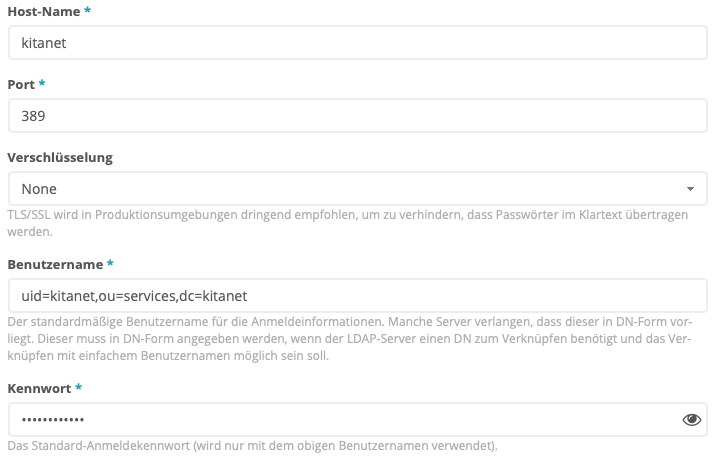
\includegraphics[width=1.0\textwidth]{res/ldapkitanet1.png}
  \caption{Teil 1 der LDAP-Konfiguration für Kitanet (Eigene Abbildung)}
  \label{fig:LDAP Kitanet Teil 1}
\end{figure}

In der Zeile \textit{Benutzername} ist ein Beispiel für eine \ac{dn} zu sehen. Für den Login im LDAP wird der Nutzer mit dem \ac{cn} \textit{admin} in dem \ac{dc} \textit{kitanet} verwendet.

\begin{figure}[h]
  \centering
  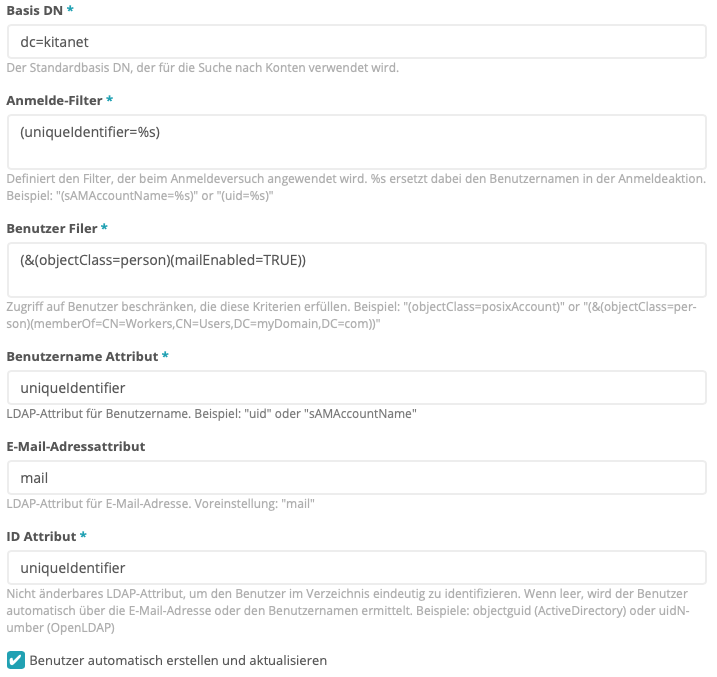
\includegraphics[width=1.0\textwidth]{res/ldapkitanet2.png}
  \caption{Teil 2 der LDAP-Konfiguration für Kitanet (Eigene Abbildung)}
  \label{fig:LDAP Kitanet Teil 2}
\end{figure}

Im unteren Teil der Einstellungen wird zunächst der \textit{Basis DN} festgelegt. Dieser legt fest in welchem Pfad des LDAP nach neuen Nutzern gesucht werden soll. Im hier vorliegenden Fall werden zunächst alle Objekte erfasst werden, sie sich in der \ac{dn} \textit{kitanet} befinden.

Der \textit{Anmelde-Filter} legt fest, welches Attribut gegen den beim Login eingegebenen Nutzernamen geprüft wird. Dies steht auch in direkter Verbindung zu den Feldern \textit{Benutzernamen Attribut} und \textit{ID Attribut} die auch beide aus dem Attribut \textit{uid} ihre Informationen beziehen. 

Das Feld \textit{Benutzer Filer} legt fest, dass nur solche Objekte in Kitanet erfasst werden die ein Attribut namens \textit{objectClass} mit dem Wert \textit{posixAccount} besitzen.

Wichtig für die hier vorliegende Problemstellung ist noch die Verknüpfung der E-Mail-Adresse des Humhub-Nutzers mit dem LDAP-Attribut \textit{mail}. 

Das Auslesen des \ac{ldap} führt somit zu nachfolgender Nutzerliste.

\begin{figure}[h]
  \centering
  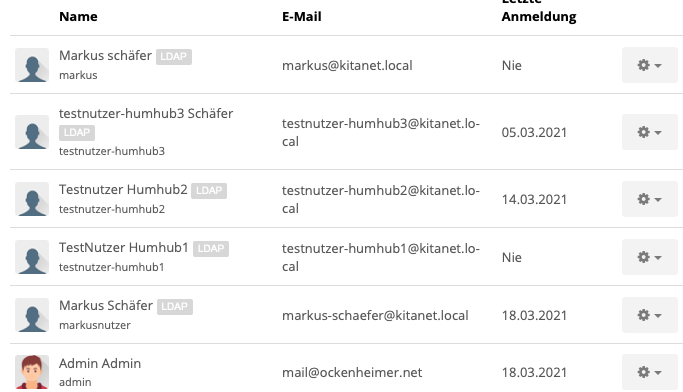
\includegraphics[width=1.0\textwidth]{res/nutzerliste.png}
  \caption{Nutzerliste der Testumgebung (Eigene Abbildung)}
  \label{fig:Nutzerliste}
\end{figure}

Das \ac{ldap} wird periodisch über einen sogenannten \textit{Cronjob} ausgelesen. Neue Nutzer werden entsprechend den oben dargestellten Kriterien angelegt und können sich ab diesem Moment mit dem in \ac{ldap} vergebenen Kennwort anmelden.

Dies schließt die Beschreibung des \textit{IST-Zustand} von Kitanet und der Testumgebung ab. Im folgenden werden nun die Grundlagen zum E-Mail-Versand dargestellt.

\chapter{Der Standard \textit{SMTP}}

Bereits in den Anfängen des \ac{arpanet} wurde die erste Software zum Versenden und Empfangen einer E-Mail zwischen Rechnern innerhalb eines Netzwerks entwickelt. \textquote{In March [1972] Ray Tomlinson at BBN wrote the basic email message send and read software, motivated by the need of the ARPAnet developers for an easy coordination mechanism. In July, Roberts expanded its utility by writing the first email utility program to list, selectively read, file, forward, and respond to messages. From there email took off as the largest network application for over a decade} \citep[][]{historyinternet}.

Hieraus entwickelte Jonathan Postel 1982 das \acf{smtp}.

Mit \ac{smtp} verband Postel den Wunsch, ein System zu schaffen, dass E-Mail unabhängig von der Transporttechnologie verlässlich und effizient transferiert \citep[vgl.][1]{rfc821}. Wie das Protokoll aufgebaut ist, wird nun anhand eines \textit{Gesprächs} zwischen zwei SMTP-Servern dargestellt und erläutert werden. Dieser Dialog wird in abgewandelter Form von Heinlein beschrieben \citep[vgl.][S. 24 ff.]{Heinlein2004}. 

\section{SMTP}

\textquote{The main purpose of SMTP is to deliver messages to user‘s mailboxes} \citep[][11]{rfc821}.
Wie von Postel formuliert, soll eine E-Mail via \ac{smtp} unabhängig vom Transportweg (\zb \ac{tcp}) von einem Nutzer versendet und vom Adressaten empfangen werden können. Sender ist in hier betrachtetem Dialog \verb+admin@kitanet+, Empfänger der E-Mail soll \verb+user@example.org+ sein. Den Datenaustausch vollziehen die SMTP-Server \verb+mail.kitanet+ als \textit{Client} und \verb+mail.example.org+ als \textit{Host}. Zur besseren Übersichtlichkeit werden Nachrichten des SMTP-Hosts mit H: eingeleitet, die des SMTP-Clients mit C:.

Das Design von \ac{smtp} sieht in seinem Kontext zwei Teilnehmer die Daten austauschen. Diese werden von ihm als \textit{Sender-SMTP} und \textit{Empfänger-SMTP} bezeichnet \citep[vgl.][2]{rfc821}. Dabei ist unabhängig, ob der Sender tatsächlich der Startpunkt für die Daten ist, oder ob der Empfänger der Endpunkt der Übertragung ist. Beide können auch nur Zwischenstationen innerhalb der Übertragung zwischen den Nutzern sein. \textquote{The receiver-SMTP may either be the ultimate destination or an intermediate} \citep[][2]{rfc821}.

Nach dem Herstellen der Verbindung meldet sich zunächst der Host:\\
\verb+H: Connected to mail.example.org+ \\ 
\verb+H: Escape Character ist '^]'+ \\
\verb+H: 220 mail.example.org SMTP Postfix on SuSE Linux 9.0 (i386)+

Der Host meldet mit Code 220 \textquote{Service ready} \citep[][38]{rfc821} dem Client, dass er zur Kommunikation bereit ist. 

Nun ist es am Client, sich zu identifizieren. \\
\verb+C: HELO mail.kitanet+ \\ 
\verb+H: 250 mail.example.org+

Mit Code 250 \textquote{Requested mail action okay, completed} \citep [][38]{rfc821} gibt der Host den Kommunikationskanal wieder frei.

Der Client meldet anschließend \\
\verb+C: MAIL FROM: <admin@kitanet>+ welches vom Host mit einem \\
\verb+H: 250 OK+ bestätigt wird.\\
Der Client verwendet den Befehl MAIL um die E-Mail-Transaktion zu starten. Er teilt dem Host mit, welchen Pfad das Datenpaket bisher genommen hat, bzw. welchen Weg eine eventuelle Antwort des Hosts nehmen muss um beim ursprünglichen Absender der Nachricht anzukommen. Postal spricht hier vom \textquote{reverse-path}. \textquote{When the list of hosts is present, it is a „reverse“ source route and indicates that the mail was relayed through each host on the list (the first host in the list was the most recent relay)}\citep[vgl.][20]{rfc821}.

Mit dem \ac{smtp}-Befehl\\
\verb+C: RCPT TO: <user@example.org>+ \\ 
und der Antwort des Hosts \\
\verb+H: 250 OK+\\
werden die einzelnen Empfänger der Mail gegenüber dem Host bekanntgegeben. Heinlein interpretiert die Antwort \verb+250 OK+ des Hosts damit, dass dieser sich für diese Nachricht \textquote{zuständig fühlt} \citep[vgl.][25]{Heinlein2004}.

Als nächstes folgt der Befehl \verb+DATA+. Die Antwort des Servers teilt dem Client zugleich mit, wie dieser anzeigen muss, wann der Datenblock übertragen wurde. Im Anschluss überträgt der Client die Nachricht und signalisiert das Ende der Daten mit dem Signal, in diesem Fall mit einem einzelnen Punkt.\\
\\
\verb+C: DATA+ \\
\verb+H: 354 End data with <CR><LF> . <CR><LF>+\\
\verb+C: Subject: Ein Betreff+ \\
\verb+C:+\\
\verb+C: Hallo Welt!+ \\
\verb+C:+\\ 
\verb+C:.+

Die Daten wurden nun vom Client an den Host übertragen. Dieser muss nun die Daten der Mail zur weiteren Verarbeitung vorbereiten und abspeichern. Als Antwort meldet er dem Client zurück, \textquote{unter welcher Kennung die E-Mail bei ihm erfolgreich gespeichert wurde} \citep[][25]{Heinlein2004}.\\
\verb+H: 250 Ok: queued as A6B701E890+ \\
Dies ist sogleich das Signal für den Client, die Mail aus seinem eigenen Speicher zu löschen, da Sie erfolgreich weitergeleitet wurde. Allerdings löscht er die Mail natürlich nur, wenn nicht die Mail nicht über einen anderen SMTP-Host an weitere Adressaten versendet werden muss.

Zum Beenden der Verbindung sendet der Client das Kommando \\
\verb+C: QUIT+, welches vom Host mit \\
\verb+H: 221 bye+ bestätigt wird. 

Hier war nur ein sehr vereinfachter Dialog zwischen Host und Client dargestellt. Postel stattete die Spezifikation mit weiteren, heute teils obsoleten, Optionen aus, wie z.B. der Möglichkeit Mails an ein Terminal zu verschicken, statt in ein Postfach \citep[vgl.][11]{rfc821} oder notwendigen Funktionalitäten wie dem Befehl EXPAND (EXPN) um die Teilnehmer einer Mailingliste anzeigen zu können \citep[vgl.][8]{rfc821}.

Auch musste der Host in der Lage sein, Verarbeitungsfehler mitzuteilen oder dem Client zu signalisieren, dass er den Empfänger nicht kannte. Der Umfang der gesamten Spezifikation würde hier den Rahmen sprengen, es sei insoweit auf \cite[][S. 37 ff.]{rfc821} verwiesen. Hier stellt Postel die möglichen Antworten für die SMTP-Kommandos dar.

SMTP in seiner Urform ist ein ASCII-basiertes System, also nur für die Weitergabe von Text spezifiziert. \textquote{The mail data may contain any of the 128 ASCII character codes}\citep[][21]{rfc821}. Entwicklungen wie MIME \citep[vgl.][]{rfc1521} lösten zwar das Problem der Datei-Anhänge, aber es entstand der Eindruck, der Veränderungs- und Erweiterungsdruck auf SMTP könnte die hohe Qualität des Standards gefährden. Man erkannte den Bedarf für einen Standard für Erweiterung von SMTP. So entstand der \ac{rfc} 1869.

\section{Enhanced SMTP}

1995 beschrieben Klensin u.a. im \ac{rfc} 1869 die \ac{esmtp}.
Sie wollten hierbei jedoch nicht einzelne Erweiterungen für SMTP beschreiben, sondern einen Rahmen schaffen, an den sich kommende SMTP-Erweiterungen orientieren können, aber auch müssen. \textquote{Rather than describing these extensions as separate and haphazard entities, this document enhances SMTP in an straightforward fashion that provides a framework in which all future extensions can be built in a single consistent way} \citep[][1]{rfc1869}. 

Gleichzeitig war es nicht ihre Absicht, es neuen Erweiterungen besonders einfach zu machen, SMTP als Unterbau zu verwenden. \textquote{This means that each and every extension, regardless of its benefits, must be carefully scrutinized [geprüft (Anm. d. Autors)] with respect to its implemetnation, deployment, and interoperability costs. In many cases, the cost of extending the SMTP serice will likely outweigh the benefit} \citep[][2]{rfc1869}. 

%\subsection{ESMTP-Framework}

Klensin u.a. führen in \ac{rfc} 1869 drei neue Faktoren in \ac{smtp} ein, um Erweiterungen des Standards zu vereinheitlichen.

\begin{itemize}
	\item{Den SMTP-Befehl \verb+EHLO+}\\
	Der Client, der \ac{esmtp} unterstützt soll den Dialog nicht mit dem Befehl \verb+HELO+, sondern mit \verb+EHLO+ (Extended HELO) einleiten, um damit zu prüfen, ob auch der SMTP-Host \ac{esmtp} unterstützt. Hierdurch ergab sich auch die Notwendigkeit, \ac{rfc} 821 zu erweitern, da als initialer Befehl nunmehr \verb+HELO+ und \verb+EHLO+ zugelassen sein mussten. Unterstützt der Host \ac{esmtp} nicht, sendet er auf den Befehl \verb+EHLO+ eine Fehlermeldung. Dies signalisiert dem Client, dass er mit dem Host nur ohne Erweiterungen sprechen kann \citep[vgl.][S. 3 ff.]{rfc1869}.
	\item{Zentrale Registrierung}\\
	Erweiterungen für \ac{esmtp} müssen zentral registriert und verwaltet werden. Hierfür sehen Klensin u.a. ein Zentralregister bei der \ac{iana} vor und schlagen zugleich die ersten Befehle vor \citep[vgl.][7]{rfc1869}. Hierbei handelt es sich um die von Postal 1982 vorgeschlagenen Befehle \verb+SEND+, \verb+SOML+, \verb+SAML+, \verb+EXPN+, \verb+HELP,+ und \verb+TURN+ \citep[für die Befehle vgl.][S. 23 ff.]{rfc821}.
	\item{erweiterte Parameter für \verb+MAIL FROM+ und \verb+RCPT TO+}\\
	Hier nehmen Klensin u.a. Bezug auf die bereits absehbaren Erweiterungen zu \ac{smtp}. \textquote{It is recognized that several of the extensions plannes for SMTP will make use of additional parameters associated with the MAIL FROM and RCPT TO command} \citep[][7]{rfc1869}. Im weiteren erläutern Sie die erforderliche Syntax für Befehle innerhalb von \verb+MAIL FROM+ und \verb+RCPT TO+ und betonen erneut die Notwendigkeit der Registrierung der Erweiterungen bei der \ac{iana}.
\end{itemize}

Durch die Erweiterungen und deren Registrierung entwickelte sich \ac{esmtp} zu einer sinnvollen Ergänzung. Dies mündete schließlich in der Übernahme des Systems in den Standard selbst \citep[vgl. u.a.][S. 7 ff]{rfc2821}.

Nachdem nun die theoretischen Grundlagen betrachtet wurden, werden im nächsten Kapitel die Anforderungen an den SMTP-Server im Rahmen des KitaNet formuliert. 





\chapter{Anforderungen/Nutzungsszenarien}

Das Formulieren von Anforderungen zu Beginn eines Projektes ist, wie im Folgenden dargestellt, von entscheidender Bedeutung. \textquote{Requirement engineering is a technical process. Writing requirements is therefore not like other kinds of writing} \citep[][77]{Hull2010}. Zunächst wird nun die Theorie kurz erläutert, bevor anschließend diese Theorie auf das vorliegende Projekt angewandt und konkrete Anforderungen an die \ac{smtp}-Software formuliert werden.

\section{Theorie des Requirement Engineering}

\subsection{Begriffsdefinition}

Die Erwartungen eines Kunden zu einem fertigen Produkt werden zu lassen, ist die zentrale Aufgabe in der Entwicklung. Ein wichtiger Schritt steht hier bereits am Anfang des Projekts: Das Formulieren der Anforderungen.
\textquote{Die Anforderungen an ein neues Softwareprodukt zu ermitteln, zu spezifizieren, zu analysieren, zu validieren und daraus eine fachliche Lösung abzuleiten bzw. ein Produktmodell zu entwickeln, gehört mit zu den anspruchsvollsten Aufgaben innerhalb der Softwaretechnik} \citep[][434]{Balzert2010}. 
Balzert verwendet hierbei den, wie er ausführt, allgemein gebräuchlichen Begriff des \ac{re} \citep[vgl.][434]{Balzert2010}, der auch in dieser Arbeit Verwendung findet. Andere, in hier zitierten Publikationen verwendete synonyme Begriffe sind \zb das \textit{Anforderungsmanagement}.
\textquote{Anforderungen sorgen dafür, dass sowohl der Kunde als auch Ihre Organisation das Produkt bekommt, das sie wirklich wünschen und benötigen} \citep[][6]{Grande2014}.

\textquote{Erst die Anforderungen geben Ihrem Projekt das Fundament, um gezielt das Ist der Lösung mit dem Soll der Anforderungen zu vergleichen und auf diese Weise nachweisbar das Projektziel zu erfüllen} \citep[Fahney und Hermann in][10]{Herrmann2013}.
Fahney und Hermann beschreiben aber auch die Risiken schlecht formulierter Anforderungen. \textquote{Hat man ein Projekt begonnen, die Anforderungen jedoch unvollständig, widersprüchlich oder mehrdeutig erhoben, so läuft man Gefahr, das „falsche“ Projekt zu machen, selbst wenn man das Projekt „richtig“ macht} \citep[Fahney und Hermann in][10]{Herrmann2013}. 
Es bleibt somit festzuhalten, dass bereits die Anforderungen sorgsam behandelt werden müssen.

Laut Balters können Projekte einige Eigenschaften besitzen, die die Anforderungsermittlung beeinflussen. 
\blockquote{\textquote{Eine Vorgehensweise, um systematisch von der Anforderungsermittlung bis zum fertigen Produktmodell zu gelangen, hängt von vielen Randbedingungen ab:
	\begin{itemize}
		\item Liegt eine Ausschreibung vor, dann gibt es in der Regel bereits ein vom Auftraggeber erstelltes Lastenheft.
		\item Beauftragt eine Fachabteilung die interne IT-Abteilung mit der Softwareherstellung, dann gibt es außer Ideen der Fachabteilung vielleicht noch keine strukturierte schriftliche Unterlage.
		\item Gibt es bereits ein eingesetztes Softwaresystem, das abgelöst oder verbessert werden soll?
		\item Ist eine Individualsoftware zu entwickeln oder sind kundenspezifische Anpassungen an Standardsoftware vorzunehmen?
		\item Handelt es sich um eine innovative Softwareentwicklung, für die es keine Vorbilder gibt?
	\end{itemize}
Diese Rahmenbedingungen beeinflussen die Methodik} \citep[][435]{Balzert2010}.}

Einen Risikobereich für das \ac{re} wird von Dahm beschrieben. Dem Autor geht es hier um Probleme bei der Kommunikation mit dem Kunden. \textquote{Dabei wird häufig unterstellt, daß diese Kommunikation problemlos erfolgt, d.h., das durch die Kommunikation selbst keine Probleme erzeugt werden} \citep[][S. 174 f.]{Dahme2000}.
Der Autor führt dies anschließend weiter aus. 

	\blockquote{\textquote{So ist es meist falsch, anzunehmen, daß \\
	1. der Anwender bei Projektbeginn genau weiß, was er will, \\
 	2. der Anwender das, wovon er weiß, daß er es will, vollständig mitteilen kann, \\
 	3. der Entwickler ausreichend verstanden hat, was der Anwender mitteilen konnte,\\
 	4. das kommunizierte Wissen ausreicht, um die vom Anwender gewollten Funktionen produzieren zu können, \\
 	5. der Anwender versteht, was der Entwickler außer den vorgelegten Beispielen noch leisten könnte,\\
 	6. der Anwender wüßte, welche Software möglich wäre, wenn der Entwickler besser über seine Bedürfnisse unterrichtet wäre} \citep[][175]{Dahme2000}.}

Eine gute und genaue Kommunikation zwischen Kunden und Entwickler ist somit auch beim Festlegen der Anforderungen unerlässlich. 
Balzert bringt es auf den Punkt. 
\textquote{Anforderungen (\textit{requirements} [Hervorhebung im Original]) legen fest, was man von einem Softwaresystem als Eigenschaft erwartet} \citep[][455]{Balzert2010}.

Für die Formulierung von Anforderungen nennt Balzert neun Regeln. Sie sollen zunächst nach \cite[][S. 100 ff.]{Pohl2007} kurz und prägnant formuliert sein und den Akteur klar benennen. Darüber hinaus sollen die Anforderungen klar überprüfbare Ziele formulieren. Sofern dies nicht möglich ist, sollen die Ziele soweit verfeinert werden, dass die Teilziele überprüft werden können. \\
Es soll ferner beschrieben werden, welchen Nutzen das Ziel verfolgt, im Beispiel ist die Verkürzung der Bearbeitungszeit genannt. Durch die Begründung des Ziels soll die Identifikation weiterer Ziele erleichtert werden, jedoch soll bei der Formulierung kein Lösungsansatz angegeben werden. Des weiteren ergänzt Balzert nach \cite[][S. 100 f.]{Rupp2007}, dass es wichtig sei, einschränkende Rahmenbedingungen mit zu benennen und die Ziele realistisch zu formulieren \citep[vgl.][S. 457 ff.]{Balzert2010}.


Balzert beschreibt verschiedene Rahmenbedingungen, die die Auswahl und Entwicklung von Software beeinflussen. \textquote{Eine \textbf{Rahmenbedingung} \textit{(constraint)} [Hervorhebungen im Original]  - auch Restriktion genannt - legt organisatorische und/oder technische Restriktionen für das Softwaresystem und/oder den Entwicklungsprozess fest}\citep[][459]{Balzert2010}.
Hierunter zählen zum Einen \textit{organisatorische Rahmenbedingungen} wie der \textit{Anwendungsbereich} oder die \textit{Zielgruppe} für die eingesetzte Software. Auch \textit{Betriebsbedingungen}, wie die tägliche Nutzungszeit des Produktes oder ob das Produkt \zb für mobiles Arbeiten vorbereitet sein muss \citep[vgl.][S. 459 f.]{Balzert2010} gehören zu den organisatorischen Rahmenbedingungen. 
Zum Anderen nennt Balzert \textit{technische Rahmenbedingungen}, die eine Software erfüllen muss, um eingesetzt werden zu können. Diese sind die \textit{technische Produktumgebung}, also auf welcher Hardware und unter welchem Betriebssystem die Software funktionieren soll und die \textit{Anforderungen an die Entwicklungsumgebung}, in denen \ua festgelegt wird, welche Schnittstellen die Software bereitstellen muss oder welche Programmierumgebung verwendet werden muss \citep[vgl.][S. 460 f.]{Balzert2010}.

Weiteren Einfluss auf die Anforderungen nimmt der Nutzungskontext. Hierunter versteht Balzert die \textquote{materielle und immaterielle Umgebung} \citep[][461]{Balzert2010} in der das Softwaresystem zum Einsatz kommt. 
Unterschieden wird hier zwischen der für das System relevante Umgebung, den \textit{Kontext}, der bei der Systementwicklung zu betrachten sei, und der durch eine \textit{Grauzone} abgegrenzten irrelevanten Umgebung, wie in der folgenden Abbildung dargestellt \citep[vgl.][462]{Balzert2010}.

\begin{figure}[h]
  \centering
  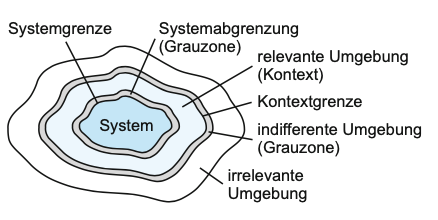
\includegraphics[width=0.8\textwidth]{res/Anforderung1.png}
  \caption{Das System und seine Umgebung \citep[][462]{Balzert2010})}
  \label{fig:Systemumgebung}
\end{figure}

Bisher wurden nur die \textit{funktionalen Anforderungen} beschrieben. Was soll das Produkt am Ende leisten, aus welchem Grund wird es entwickelt? Daneben gibt es eine weitere Art, nämlich die \textit{nichtfunktionalen Anforderungen}. \\ \textquote{\textbf{Nicht-funktionale Anforderungen} [Hervorhebung im Original] lassen sich qualitativ unterscheiden in \\
- Qualitätsattribute der gewünschten Funktionen \\ 
- Anforderungen an das implementierte System als Ganzes, \\ 
- Vorgaben für die Durchführung des Systemerstellung \\ 
- Anforderungen an Prüfung, Einführung, Betreuung und Betrieb} \citep[][S. 27 f.]{Partsch2010}.
Hierunter fallen somit sämtliche Aspekte, die nicht direkt einer Anforderung zuzuordnen sind, sondern das Produkt als ganzes betreffen \citep[vgl.][463]{Balzert2010}. Balzert nennt in diesem Zusammenhang \textquote{\ua Genauigkeit, Verfügbarkeit, Nebenläufigkeit, Konsumierbarkeit (eine Obermenge der Benutzbarkeit),[...], Zuverlässigkeit, Sicherheit, Service-Anforderungen, Support [...]} \citep[][463]{Balzert2010}. 
Partsch gibt im weiteren zu Bedenken, dass nichtfunktionale Anforderungen zumeist \textquote{wenn überhaupt, dann meist nicht präzise formuliert [werden]} \citep[][30]{Partsch2010}. Er begründet dies mit der Aussage bezüglich der Anforderung \textquote{(„Das weiß man ja“)} \citep[][30]{Partsch2010}.

Während die funktionalen Anforderungen beschreiben \textit{was} ein Produkt leisten muss, beschreiben nicht-funktionale Anforderungen \textit{wie} diese Leistung erbracht werden soll \citep[vgl.][30]{Partsch2010}.

\subsection{Priorisierung}

Anforderungen an ein Produkt sind nie gleichwertig zueinander. 
\textquote{Some requirements are non-negotiable. If they are not met, the product is of no use} \citep[][83]{Hull2010}. Wie die Priorisierung der Anforderungen gestaltet werden kann, wird nun kurz dargestellt.

Hull u.a. schlagen vor, Anforderungen mit verschiedenen Werten auszustatten. Sie beschreiben in einem Beispiel die Werte M (mandatory limit), D (desired value) und B (best value) \citep[vgl.][83]{Hull2010}. \textquote{These three values can be held in separate attributes, or represented within the text in a labelled form, such as „The system shall support [M:50, D:100, B:200] simultaneous users“} \citep[][83]{Hull2010}.
Diese Methode gibt einzelnen Anforderungen eine gewisse Flexibilität, indem die Grenze für das Erreichen des Zieles klarer herausgestellt ist. Im genannten Beispiel sind 50 gleichzeitige Nutzer die Mindestgrenze, 100 Nutzer sind erstrebenswert, bestenfalls sind 200 gleichzeitige Nutzer möglich. Unterstützt die Lösung nun nur 99 Nutzer, \textquote{then it is most likely still of some value to the customer} \citep[][83]{Hull2010}.

Eine Aussage über die Wertigkeit der Anforderungen zueinander wird hier jedoch nicht getroffen. 

%Zur Lösung dieses Problems schlägt Balzert vor, die Anforderungen nach Ihrer Wichtigkeit zu bewerten. Er gibt dabei jedoch zu bedenken, dass Wichtigkeit von unterschiedlichen Seiten betrachtet werden kann. \textquote{Wichtigkeit bezogen auf die Funktionalität des Systems, Wichtigkeit bezogen auf die Benutzerfreundlichkeit, Wichtigkeit bezogen auf die frühzeitige Verfügbarkeit usw} \citep[][543]{Balzert2010}. Auch seien andere Kriterien wie \zb Kosten oder dem verursachten Schaden bei Nichtberücksichtigung denkbar \citep[vgl.][543]{Balzert2010}.

Das \ac{ieee} ist eine der Institutionen, die sich mit der Standardisierung technischer Vorgänge beschäftigen. Ähnlich den bereits erwähnten \ac{rfc}, die unter der Schirmherrschaft der \ac{ietf} verwaltet werden, gibt das \ac{ieee} Standardisierungsvorschriften heraus. Eine dieser Schriften, die \ac{ieee} Std 830-1998, beschreibt die empfohlene Vorgehensweise bei der Spezifikation von Software Anforderungen (\ac{srs}).

In besagtem Standard schlägt das \ac{ieee} vor, die Anforderungen nach ihrer Notwendigkeit einzuordnen. \textquote{Another way to rank requirements is to distinguish classes of requirements as essential, conditional, and optional} \citep[][7]{ieee1998}. Balzert steht dieser Einordnung kritisch gegenüber. \textquote{Erfahrungen haben gezeigt, dass die Verwendung dieser Ausprägungen dazu führt, dass die meisten Anforderungen mit \textbf{essenziel} [Hervorhebung im Original] gekennzeichnet werden, während optionale Anforderungen nur selten vorkommen} \citep[][543]{Balzert2010}.

Als Alternative schlägt Balzert die Verwendung des Kano-Modells vor. Dieses Modell bezieht sich auf die \textit{Theory of Attractive Quality} des japanischen Professors Noriaki Kano, dessen Studien einen Zusammenhang zwischen dem Erfüllen von Qualitätsmerkmalen einerseits und der Kundenzufriedenheit andererseits belegen \citep[vgl.][77]{Hoelzing2008}. \textquote{Durch eine Kundenbefragung im Rahmen einer Produktentwicklung werden nur geringfügige Mängel an den bisher angebotenen Modellen festgestellt. Daraus wird die Annahme abgeleitet, dass der Schlüssel zum Erfolg in eher latenten, nicht explizit artikulierten oder bewussten Kundenbedürfnissen liegt} \citep[][78]{Hoelzing2008}. Hölzing beschreibt im weitern wie Kano fünf Qualitätsattribute herausarbeitet \citep[vgl.][82]{Hoelzing2008}. Drei dieser fünf Eigenschaften bespricht dann auch Balzert.
\textquote{Die Produkteigenschaften werden in Kategorien eingeteilt:\\
- \textbf{Basiseigenschaften:} Vom Kunden selbstverständlich vorausgesetzte Eigenschaften (implizite Erwartung). Fehlt eine Basiseigenschaft, dann entsteht Unzufriedenheit. Werden sie erfüllt, dann entsteht aber \textit{keine} Zufriedenheit. \\
- \textbf{Leistungseigenschaften:} Vom Kunden bewusst geforderte Eigenschaften (Sonderausstattung!). Sie schaffen beim Kunden Zufriedenheit bzw. beseitigen Unzufriedenheit - je nach Ausmaß. \\
- \textbf{Begeisterungseigenschaften:} Eigenschaften die der Kunde \textit{nicht} erwartet hat. Die Kundenzufriedenheit wächst überproportional, wenn die Eigenschaft vorhanden ist [alle Hervorhebungen im Original]} \citep[][544]{Balzert2010}.

Die nicht durch Balzert benannten Eigenschaften sind von Hölzing nach Kano beschrieben. Es handelt sich um \textit{indifferent quality elements}, also Eigenschaften des Produktes, die weder Zufriedenheit noch Unzufriedenheit beim Kunden auslösen, sowie \textit{reverse quality elements}, welche eine höhere Zufriedenheit beim Kunden auslösen, je schlechter sie die Erwartungen des Kunden erfüllen \citep[vgl.][83]{Hoelzing2008}.

Das Verhältnis der Kundenzufriedenheit im Verhältnis zum Erfüllungsgrad der jeweiligen Produkteigenschaft ist in der folgenden Grafik visualisiert.

\begin{figure}[h]
  \centering
  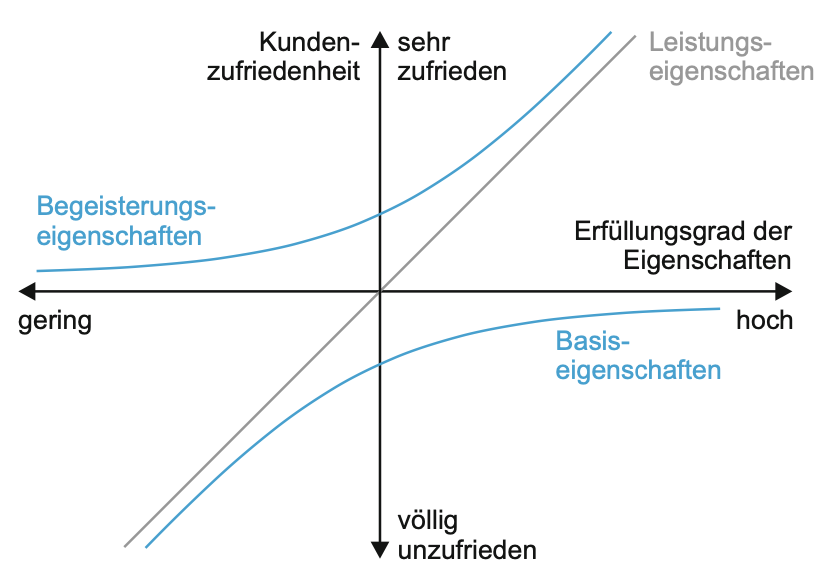
\includegraphics[width=0.8\textwidth]{res/kano.png}
  \caption{Die Entwicklung der Kundenzufriedenheit im Kano-Modell \citep[][545]{Balzert2010})}
  \label{fig:Kanomodell}
\end{figure}

Es wurden nun verschiedene Ansätze der Priorisierung und Wertung von Anforderungen besprochen. Der Autor dieser Bacherlorarbeit ist im Rahmen seiner Tätigkeit bereitts mit der Unterteilung der \ac{ieee} vertraut. Aus eigener Erfahrung kann er die Kritik von Balzert durchaus nachvollziehen, ist sich jedoch sicher, die Anforderungen sinnvoll abstufen zu können. Für die Priorisierung dern Anforderungen pm Rahmen dieses Projekts sollen daher die Voragben der \ac{ieee} genutzt werden.

In der Folge wird nun das erarbeitete Wissen auf das vorliegende Projekt angewandt und die Anforderungen formuliert. 


\section{Anforderungen}
Beschreibt die Anforderungen an den SMTP-Server, z.B.:
\begin{itemize}
	\item Lauffähig auf Ubuntu
	\item Zusammenarbeit mit LDAP
	\item Automatisierung der Nutzerverwaltung
	\item Gute Dokumentation
	\item geringer (im besten Fall gar kein) Wartungsaufwand
	\item Kostengünstig
	\item etc.
\end{itemize}


\section{Nutzungsszenarien}
Welche Szenarien soll der \ac{mta} abdecken? Welche Funktionen sind notwendig (\zb nur interne Mails, keine Erreichbarkeit von außen)? Was ist bei der Lizenzierung zu beachten? Gibt es weitere wichtige Aspekte? Der SMTP-Server soll mit dem eingesetzten IMAP-Client Dovecot zusammenarbeiten.
\section{Testfälle}
Aufgrund der beschriebenen Nutzungsszenarien werden Testfälle formuliert, die den Erfolg des Projektes kennzeichnen. 

\chapter{Zur Auswahl stehende SMTP-Software}
Vergleich von SMTP-Server-Software für den Einsatz auf Ubuntu. 
\section{postfix}
Erfüllt die Software die gestellten Anforderungen? Was spricht gegen einen Einsatz?
\section{EmailSuccess}
Inhaltlich wie oben.

\chapter{Entscheidung}
Welche SMTP-Software wurde gewählt? 

\chapter{Installation und Tests}

\section{Einrichtung und Anbindung SMTP an LDAP}
Wie steuert das \ac{ldap} den SMTP-Server? Wie funktioniert der Informationsaustausch (neue Nutzer, etc)?

\section{Tests}
Allgmeines zu den durchgeführten Tests. Kam es zu Problemen bei der Testung?
\subsection{Dokumenation der einzelnen Tests}
Wurde der Test bestanden? Musste der Test unerwartet an die Gegebenheiten angepasst werden?

\chapter{Fazit}

\blindtext





\newpage

% nocite lässt alle Werke anzeigen, auch solche die nicht verlinkt sind.
%\nocite{*}
\printbibliography[heading=none]

\newpage

% Rudi will kein Abbildungsverzeichnis
\listoffigures
%\listoftables
%\listlistoflistings
\newpage
%\cleardoublepage
%!TEX root = ../bachelorthesis.tex
\appendix
\renewcommand\chaptername{Anhang}


\chapter{Anforderungsdokument}
\markboth{A. Ein Anhang}{}
\label{ch:Anhang}

\section{Einführung}
\subsection{Zweck des Dokuments}
Dieses Dokument definiert die Anforderungen an das Projekt "Einführung eines SMTP-Servers". 
Dieses Dokument richtet sich an Entwickler die mit diesem Projekt betraut sind.

\subsection{Umfang}
Die zu installierende Software soll einen SMTP-Server bereitstellen, um E-Mail-Kommunikation innerhalb des Netzwerks der Einrichtung zu ermöglichen (vgl. RFC 821). Der Mailverkehr wird zunächst nur innerhalb des eigenen Netzwerks gewährleistet. Eine Öffnung nach außen ist zukünftig angestrebt, aber zunächst nicht Teil des Projekts.

\subsection{Definitionen, Akronyme, Abkürzungen}
\label{ch:Definition}
Eine Liste von Abkürzungen, die in diesem Dokument verwendet werden.
\begin{itemize}
	\item LDAP - Lightweight Directory Access Protocol
	\item LTS - Long Time Support
	\item RFC - Request for Comments
	\item SMTP - Simple Mail Transfer Protocol
\end{itemize}

Die Anforderungen werden in drei Stufen der Notwendigkeit unterschieden und entsprechend priorisiert. Die Zugehörigkeit der Anforderung zu den Stufen werden mit der Formulierung der Anforderung angezeigt.\\
Anforderungen beginnend mit:
\begin{itemize}
	\item \textit{Das System muss} oder \textit{Das System darf keine} gehören zur höchsten Stufe.
	\item \textit{Das System soll} oder \textit{Das System darf} gehören zur mittleren Stufe.
	\item \textit{Das System kann} gehören zur niedrigen Stufe.
\end{itemize}

\subsection{Referenzen}
Referenzierte Dokumente, die in diesem Dokument verwendet werden.
\begin{itemize}
	\citereset
	\item RFC 821 \\
	https://tools.ietf.org/html/rfc821 
	\item RFC 2821\\
	https://tools.ietf.org/html/rfc2821
	\citereset
\end{itemize}



\subsection{Übersicht}
Dieses Anforderungsdokument enthält die Anforderungen und Spezifikationen, die an den SMTP-Server gestellt werden.
Sie dienen als Entscheidungsgrundlage für die anzuschaffende Software.

\section{Produktübersicht}
\subsection{Produktperspektive}
Das finale System bildet eine virtuelle Maschine (im weiteren \textit{der Server}) innerhalb eines QNAP-NAS mit 4GB Arbeitsspeicher.
Auf dem Server wird als Betriebssystem Ubuntu 20.04 LTS eingesetzt. Auf diesem System wird ebenfalls folgende relevante Software eingesetzt:
\begin{itemize}
	\item Open-LDAP ver. 2.4.49
	\item Apache2 ver. 2.4.41
	\item Dovecot ver. 2.3.7.2
	\item PHP ver. 7.4
\end{itemize} 
Der Server ist für Laptops innerhalb des Netzwerks erreichbar. Ein direkter Zugriff zur Hardware ist grds. nicht vorhanden.

Die Software ist erreichbar über Port 25 des Servers.  

\subsection{Produktfunktionen}
Die Software verwaltet die Entgegennahme und Auslieferung von Datenpaketen mit dem IMAP-Client Dovecot.
Zur Ermittlung bekannter Mail-Adressen gleicht die Software ihren Bestand mit dem lokalen \ac{ldap} ab.
Die Software besitzt den vollen Funktionsumfang von \ac{smtp} (vgl. RFC 2821).

\subsection{Nutzereigenschaften}
Der Nutzer hat keine direkte Interaktion mit der Software. Kontakt besteht ausschließlich mittelbar und automatisiert über den IMAP-Client Dovecot
\subsection{Einschränkungen}
Die Software teilt sich den vorhandenen Arbeitsspeicher mit einer per PHP realisierten Webseite und einem LDAP-Server. Somit darf die durchschnittliche RAM-Belegung nicht größer als 512 MB sein.
\subsection{Annahmen und Abhängigkeiten}
Das System bleibt zumindest bis April 2022 auf dem Betriebssystem Ubuntu 20.04 LTS. Sollte ein Plattformwechsel angestrebt werden, muss vorher die Funktionalität getestet werden.
\subsection{verzögerte Anforderungen}
keine 
\section{Spezifische Funktionen}

\subsection{externe Schnittstellen}
\subsubsection{Benutzerschnittstellen}
Nicht vorgesehen.
\subsubsection{Hardwareschnittstellen}
Nicht vorgesehen.
\subsubsection{Softwareschnittstellen}
Nicht vorgesehen.
\subsubsection{Kommunikationsschnittstellen}
Erreichbarkeit über Port 25 zum Austausch von \ac{lmtp}-Befehlen mit IMAP-Client auf dem selben System. Die Öffnung des Ports nach außen soll für zukünftigen Austausch von \ac{smtp}-Befehlen mit entfernten \ac{smtp}-Servern vorgesehen werden.
\subsection{Funktionen}
\subsubsection{(E)SMTP-Kommunikation}
\textbf{Zweck der Funktion} \\
Das System muss (E)\ac{smtp}- und \ac{lmtp}-Befehle entgegennehmen und verarbeiten. \\
\textbf{Auslösung/Reaktion der Funktion} \\
Auslösung: \\
Kontaktaufnahme durch Zugriff anderer Programme auf Port 25\\
Reaktion:\\
Prozess Einleitung des (E)SMTP-Protokolls MAIL gem. S.4 RFC 821 \\
\textbf{Mit Funktion verbundene Anforderungen} \\
Versenden und Empfangen von E-Mails werden ermöglicht.\\
\subsubsection{Abgleich LDAP}
\textbf{Zweck der Funktion} \\
Das System soll einen aktuellen Datenbestand über im LDAP angelegte Empfänger besitzen.\\
\textbf{Auslösung/Reaktion der Funktion} \\
Auslösung:\\
Automatisierte Anstoß zur Aktualisierung der Daten.\\
Reaktion:\\
Aufnahme neuer Empfänger, Löschung von nicht existenten Adressen.\\
\textbf{Mit Funktion verbundene Anforderungen}\\
Es werden nur Mails von Empfängern verarbeitet, die in der Datenbank des LDAP erfasst sind.\\
\subsection{Leistungsanforderung}
Das System soll Mails so schnell wie möglich, jedoch in maximal 15 Sekunden beim Empfänger abliefern. Eine Echtzeit-Verarbeitung ist nicht notwendig.\\
Das System soll 100\% der Mails beim jeweiligen Empfänger abliefern.\\
Das System soll in der Lage sein, mindestens 10 Mails gleichzeitig verwalten und korrekt zustellen zu können.\\
Das System soll Mails mit Dateianhängen bis zu 25 MB verarbeiten können.\\
\subsection{Design-Einschränkungen}
Das System muss mit dem \ac{imap}-Client Dovecot zusammenarbeiten.
\subsection{Softwaresystem-Eigenschaften}
\textbf{Zuverlässigkeit} \\
Das System muss nach einem Neustart des Servers ohne Nutzerzutun automatisch starten.\\
\textbf{Verfügbarkeit} \\
Das System soll jederzeit zur Verfügung stehen\\
\textbf{Sicherheit} \\
Das System soll einen unberechtigten Zugriff Dritter auf die verarbeiteten E-Mails verhindern.\\
\textbf{Wartbarkeit} \\
Das System soll, ohne Veränderung der Systemumgebung, Wartungsfrei sein.\\
Das System soll über eine detaillierte Dokumentation verfügen.\\
\textbf{Portierbarkeit} \\
Das System soll grundsätzlich auf andere Plattformen portierbar sein.\\

\subsection{andere Anforderungen}
\subsubsection{Anschaffungskosten}
Das System darf keine Anschaffungskosten auslösen.
\subsubsection{Betriebskosten}
Das System darf keine laufenden Betriebskosten durch Lizenzierung o.ä. auslösen.


\chapter{Testfälle}
\label{ch:Testfaelle}

\section{Testreihe 1 Versenden einer Mail}
\subsection{Testfall 1.1}
\begin{itemize}
	\item Testgegenstand:\\
	Versenden einer E-Mail an einen existierenden Empfänger
	\item Testkonfiguration:\\
	System ohne Last\\
	Mail-Sender \verb+mail@kitanet.local+ in System angelegt\\
	Mail-Empfänger \verb+testnutzer@kitanet.local+ in System angelegt
	\item Testbeschreibung:\\
	Versenden einer E-Mail über Dovecot-Client mit Nutzer \verb+mail@kitanet.local+ \\ an \verb+testnutzer@kitanet.local+
	\item Bezug:\\
	Anforderung \textit{(E)SMTP-Kommunikation}
	\item Priorität:\\
	unbedingt erforderlich
	\item Details:\\
	Stellt sicher, dass Mails über den Server versendet werden können (Grundfunktionalität System)
	\item Soll-Ergebnis:\\
	E-Mail geht in Postfach des Empfängers ein.
	\item Ist-Ergebnis:\\
	\item Bestanden:\\
	\item Aus welcher Phase stammt der Fehler:\\
	\item Kommentar:\\
	\item Tester:\\
	\item Datum/Uhrzeit:\\
\end{itemize}

\subsection{Testfall 1.2}
\begin{itemize}
	\item Testgegenstand:\\
	Versenden einer E-Mail an einen nicht existierenden Empfänger
	\item Testkonfiguration:\\
	System ohne Last\\
	Mail-Sender \verb+mail@kitanet.local+ in System angelegt\\
	Mail-Empfänger \verb+foobar@kitanet.local+ nicht in System angelegt
	\item Testbeschreibung:\\
	Versenden einer E-Mail über Dovecot-Client mit Nutzer \verb+mail@kitanet.local+ \\ an \verb+foobar@kitanet.local+
	\item Bezug:\\
	Anforderung \textit{(E)SMTP-Kommunikation}
	\item Priorität:\\
	nachgeordnet
	\item Details:\\
	Test provoziert SMTP-Fehlermeldung 550
	\item Soll-Ergebnis:\\
	Sender erhält SMTP-Fehlermeldung 550 oder äquivalente Rückmeldung des Servers \citep[vgl.][16]{rfc821}.
	\item Ist-Ergebnis:\\
	\item Bestanden:\\
	\item Aus welcher Phase stammt der Fehler:\\
	\item Kommentar:\\
	\item Tester:\\
	\item Datum/Uhrzeit:\\
\end{itemize}

\section{Testreihe 2 LDAP-Anbindung}
\subsection{Testfall 2.1}
\begin{itemize}
	\item Testgegenstand:\\
	Anlegen eines Benutzers via LDAP und Versenden einer Test-Mail
	\item Testkonfiguration:\\
	ruhendes System\\
	Mail-Sender \verb+mail@kitanet.local+ in System angelegt\\
	Mail-Empfänger \verb+ldap-test3@kitanet.local+ nicht in System angelegt
	\item Testbeschreibung:\\
	Nutzer mit LDAP-Attribute \verb+mail = ldap-test3@kitanet.local+ wird im System angelegt\\
	Wartezeit bis Datenaustausch zwischen LDAP und SMTP-Server stattgefunden hat. (ggf. manuelles Anstoßen des Cronjobs)\\
	Versenden einer E-Mail über Dovecot-Client mit Nutzer \verb+mail@kitanet+ \\ an \verb+ldap-test3@kitanet.local+
	\item Bezug:\\
	Anforderung \textit{LDAP-Anbindung}
	\item Priorität:\\
	hoch
	\item Details:\\
	Neue Benutzer sollen E-Mail-Funktionalität ohne Eingreifen des Administrators nutzen können.\\
	Manuelles Auslösen des Cronjobs erspart Wartezeit.
	\item Soll-Ergebnis:\\
	E-Mail geht in Postfach des Empfängers ein.
	\item Ist-Ergebnis:\\
	\item Bestanden:\\
	\item Aus welcher Phase stammt der Fehler:\\
	\item Kommentar:\\
	\item Tester:\\
	\item Datum/Uhrzeit:\\
\end{itemize}

\subsection{Testfall 2.2}
\begin{itemize}
	\item Testgegenstand:\\
Löschen eines Benutzers via LDAP und Versenden einer Test-Mail
	\item Testkonfiguration:\\
	Testfall 2.1 wurde erfolgreich durchgeführt\\
	System ruht\\
	Keine Änderung der Konfiguration
	\item Testbeschreibung:\\
	Löschung des Nutzers mit LDAP-Attribut: \verb+mail = ldap-test3@kitanet.local+\\
	Wartezeit bis Datenaustausch zwischen LDAP und SMTP-Server stattgefunden hat. (ggf. manuelles Anstoßen des Cronjobs)\\
	Versenden einer E-Mail über Dovecot-Client mit Nutzer \verb+mail@kitanet.local+ \\ an \verb+ldap-test3@kitanet.local+
	\item Bezug:\\
	Anforderung \textit{LDAP-Anbindung}
	\item Priorität:\\
	hoch
	\item Details:\\
	Löschen alter Nutzer verringert Speicherbedarf auf den Servern
	\item Soll-Ergebnis:\\
	Sender erhält SMTP-Fehlermeldung 550 oder äquivalente Rückmeldung des Servers \citep[vgl.][16]{rfc821}.
	\item Ist-Ergebnis:\\
	\item Bestanden:\\
	\item Aus welcher Phase stammt der Fehler:\\
	\item Kommentar:\\
	\item Tester:\\
	\item Datum/Uhrzeit:\\
\end{itemize}



\section{Systemausfall und Neustart}
\subsection{Testfall 3.1}
\begin{itemize}
	\item Testgegenstand:\\
Kontrollierter Neustart des Systems
	\item Testkonfiguration:\\
	System ruht
	\item Testbeschreibung:\\
	Verbindung zu Server via \verb+SSH+
	Befehl zum Neustart wird erteilt (\verb+sudo reboot+)
	Nachdem Weboberfläche von \textit{KitaNet} wieder erreichbar ist, wird Testfall 1.1 wiederholt.
	\item Bezug:\\
	Anforderung \textit{Zuverlässigkeit}
	\item Priorität:\\
	unbedingt erforderlich
	\item Details:\\
	Aufwand für Wiederinbetriebnahme des Systems soll so gering wie möglich gehalten werden. SMTP-Software soll selbstständig starten.
	\item Soll-Ergebnis:\\
	Wiederholung von Testfall 1.1 wird erfolgreich durchgeführt
	\item Ist-Ergebnis:\\
	\item Bestanden:\\
	\item Aus welcher Phase stammt der Fehler:\\
	\item Kommentar:\\
	\item Tester:\\
	\item Datum/Uhrzeit:\\
\end{itemize}

\subsection{Testfall 3.2}
\begin{itemize}
	\item Testgegenstand:\\
Neustart des Systems nach unkontrollierter Abschaltung
	\item Testkonfiguration:\\
	System ruht
	\item Testbeschreibung:\\
	Trennung des Systems von Stromzufuhr (Stromstecker raus)\\
	Wiederverbindung mit Stromzufuhr\\
	Manueller Neustart des Systems\\
	Nachdem Weboberfläche von \textit{KitaNet} wieder erreichbar ist, wird Testfall 1.1 wiederholt.
	\item Bezug:\\
	Anforderung \textit{Zuverlässigkeit}
	\item Priorität:\\
	unbedingt erforderlich
	\item Details:\\
	System muss nach Stromausfall ohne Eingriff eines Administrators wieder eigenständig  funktionieren.
	\item Soll-Ergebnis:\\
	Wiederholung von Testfall 1.1 wird erfolgreich durchgeführt
	\item Ist-Ergebnis:\\
	\item Bestanden:\\
	\item Aus welcher Phase stammt der Fehler:\\
	\item Kommentar:\\
	\item Tester:\\
	\item Datum/Uhrzeit:\\
\end{itemize}


\chapter{Dateien und Datenbankeinträge aus Kitanet}
\begin{lstlisting}[caption={Ergebnis der LDAP-Abfrage für den Nutzer 'administrator'}, label={ldapabfrage}]
Enter LDAP Password:
dn: uniqueIdentifier=administrator,ou=people,dc=kitanet
mailAlias: admin@kitanet.local
mailAlias: kitanet@kitanet.local
mailAlias: postmaster@kitanet.local
cn: admin
objectClass: organizationalPerson
objectClass: person
objectClass: top
objectClass: PostfixBookMailAccount
objectClass: extensibleObject
mailUidNumber: 5000
givenName: admin
mailEnabled: TRUE
mailGidNumber: 5000
sn: kitanet
mailQuota: 10240
uniqueIdentifier: administrator
userPassword:: e0NSWVBUfSQ2JGZQbGNTaHVaJEpXRnpRcklyT0FNZ2pWN3ZkT1hhekhiZ3JhQ3B
 MVUlsUFo0OHFCQVpZQ3FDL2MyY0liVkZISmpFT0p1VVJuRU1jeHpnS2Q0WFplR0hNNE84ZFdwREIv
mail: administrator@kitanet.local
mailHomeDirectory: /srv/vmail/administrator@kitanet.local
mailStorageDirectory: maildir:/srv/vmail/administrator@kitanet.local/Maildir
\end{lstlisting}
\newpage
\begin{lstlisting}[caption={/etc/postfix/main.cf}, label={postfix/main.cf}]
### Base Settings
# Listen on all interfaces
	inet_interfaces = all
# Use TCP IPv4 and IPv6
	inet_protocols = all
# Greet connecting clients with this banner
	smtpd_banner = $myhostname ESMTP $mail_name (Ubuntu)
# Fully-qualified hostname
	myhostname = mail.kitanet.local
# Trusted networks/hosts (these are allowed to relay without authentication)
	mynetworks =
    # Local
    localhost
    127.0.0.0/8
    # External
    192.168.4.0/24


### Local Transport
	# Disable local transport (so that system accounts can not receive mail)
		local_transport = error:NO LOCAL
	# Do not use local maps for alias
		alias_maps = 
	# Local domain (could be omitted, since it is automatically derived from $myhostname)
		mydomain = example.com
	# Mails for these domains will be transported locally
		mydestination =
		  $myhostname
		  localhost.$mydomain
		  localhost
# Virtual Reciepients
	# Deliver mail for virtual recipients via Dovecot
		virtual_transport = dovecot
	# Process one mail at one time
		dovecot_destination_recipient_limit = 1
	# accepted virtual domains
		virtual_mailbox_domains = hash:/etc/postfix/virtual_domains
	# accepted virtual recipients
		virtual_mailbox_maps = proxy:ldap:/etc/postfix/ldap_virtual_recipients.cf
	# accepted aliases
		virtual_alias_maps = proxy:ldap:/etc/postfix/ldap_virtual_aliases.cf


### ESMTP 
# SASL
# Enable SASL (required for SMTP authentication)
	smtpd_sasl_auth_enable = yes

### Session Policies  
# Who could receive mails
	smtpd_recipient_restrictions =
    reject_non_fqdn_recipient
    reject_unknown_recipient_domain
  # Allow relaying for SASL authenticated clients and trusted hosts/networks
  # This can be put to smtpd_relay_restrictions in Postfix 2.10 and later 
  	permit_sasl_authenticated
  	permit_mynetworks
  # If not authenticated or on mynetworks, reject mailing to external addresses
 	 reject_unauth_destination
  # Reject the following hosts
  # maybe never used
    check_sender_ns_access cidr:/etc/postfix/drop.cidr
    check_sender_mx_access cidr:/etc/postfix/drop.cidr
  # Finally permit (relaying still requires SASL auth)
  # WARNING: Due to this permit, everyone will be able to send emails to internal addresses without authentication. If this is set to reject though, the server does not receive emails from external addresses. Unfortunately I do not have a solution for this.
	  permit
# Reject the request if the sender is the null address and there are multiple recipients
	smtpd_data_restrictions = reject_multi_recipient_bounce
# who could send mails
	smtpd_sender_restrictions =
    reject_non_fqdn_sender
    reject_unknown_sender_domain
# HELO/EHLO Restrictions
	smtpd_helo_restrictions =
		# mynetworks can communicate with SMTP
      permit_mynetworks
    # look for identitycheck to prevent Hostname abuse
    # maybe never used, but you never know
      check_helo_access pcre:/etc/postfix/identitycheck.pcre
    #reject_non_fqdn_helo_hostname
      reject_invalid_hostname
# Deny VRFY recipient checks
	disable_vrfy_command = yes
# Require HELO
	smtpd_helo_required = yes
# Reject instantly if a restriction applies (do not wait until RCPT TO)
	smtpd_delay_reject = no
# Reject the following Clients (Blacklist)
	smtpd_client_restrictions = check_client_access cidr:/etc/postfix/drop.cidr
\end{lstlisting}

\begin{lstlisting}[caption={/etc/postfix/ldap\_virtual\_recipients.cf}, label={postfix/recipients.cf}]
	bind = yes
# LDAP-User
	bind_dn = uid=postfix,ou=services,dc=kitanet
# LDAP-User-PW
	bind_pw = postfix
# LDAP-Server
	server_host = ldap://127.0.0.1:389
# part of tree, where to search for users
	search_base = ou=people,dc=kitanet
# fqdn for users
	domain = kitanet.local
# LDAP-Query to find the users
# %s is the variable representing the "RCPT TO:" adress
	query_filter = (&(mail=%s)(mailEnabled=TRUE))
# which attribute should be returned
	result_attribute = mail
\end{lstlisting}

\begin{lstlisting}[caption={/etc/postfix/ldap\_virtual\_aliases.cf}, label={postfix/aliases.cf}]
	bind = yes
# LDAP-User
	bind_dn = uid=postfix,ou=services,dc=kitanet
# LDAP-User-PW
	bind_pw = postfix
# LDAP-Server
	server_host = ldap://127.0.0.1:389
# part of tree, where to search for users
	search_base = ou=people,dc=kitanet
# fqdn for users
	domain = kitanet.local
# LDAP-Query to find the users
# %s is the variable representing the "RCPT TO:" adress
	query_filter = (&(mailAlias=%s)(mailEnabled=TRUE))
# which attribute should be returned
	result_attribute = mail
\end{lstlisting}
\begin{lstlisting}[caption={/etc/postfix/sasl/smtpd.conf}, label={postfix/sasl}]
log_level: 3
pwcheck_method: saslauthd
mech_list: PLAIN LOGIN
\end{lstlisting}



%%!TEX root = ../hausarbeit.tex
% Erklaerung der Selbststaendigkeit.
% Footer wird in config.tex durch \AtEndDocument{\ofoot{}} angepasst
\chapter*{Erklärung der Selbständigkeit}
\markboth{}{}
\addcontentsline{toc}{chapter}{Erklärung der Selbständigkeit}

Ich versichere, dass ich die vorliegende schriftliche Prüfungsleistung selbständig verfasst, keine anderen als die angegebenen Quellen und Hilfsmittel verwendet habe und die Stellen, die anderen Werken im Wortlaut oder dem Sinn nach entnommen sind, im Text jeweils mit Quellenbelegen kenntlich gemacht habe. Die Arbeit ist noch nicht anderweitig für Prüfungszwecke vorgelegt worden.
\\
\\
\\
\\
\\

%\begin{minipage}[c]{15,4cm}
\parbox{6cm}{\centering  \ortderarbeit, \today\hrule\strut\centering\footnotesize Ort, Datum}
\hfill
\vspace{-2cm}
\parbox{6cm}{\centering {\color{white} X} \hrule\strut \centering\footnotesize Unterschrift}
%\end{minipage}



%\vspace{-2cm} %hochschieben
%\includegraphics[width=0.4\textwidth,heigth=12pt]{res/Unterschrift.png}
%\vspace{2cm} % wieder runter


\end{document}

